%=====================================================================================
%
%                    1. ITERACE 
%
%
%======================================================================================
% MODELY 1. ITERACE %
% === FRONT PAGE ===
\thispagestyle{plain}
	\newgeometry{left=2cm,right=2cm,top=1.5cm}
	\pagenumbering{gobble}
	\begin{center}
		\Huge
		VYSOKÉ UČENÍ TECHNICKÉ V BRNĚ \\
			\vspace{\stretch{0.150}}


	
\includegraphics[width=\textwidth]{resources/fit-logo.pdf}
			\vspace{\stretch{0.300}}



		\Large{Projekt do předmětu AIS \\ ~ \\}
		
		\LARGE
		\textsc{Modely --- 1. iterace}
			\vspace{\stretch{0.618}}

	\end{center}

	\noindent \textbox{20. listopadu, 2017} \textbox{\hfill \textbf{Autoři:}  Daniel Dušek ~~(xdusek21) ~~~}
	\noindent \textbox{\hfill} \textbox{\hfill Filip Kalous ~~~(xkalou03) ~~~}
	\noindent \textbox{\hfill} \textbox{\hfill Anna Popková (xpopko00)~~~}

	\clearpage
	\restoregeometry

\newpage

\normalsize

\newpage
\section*{Diagram případu použití}
\begin{figure}[h!]
\begin{center}
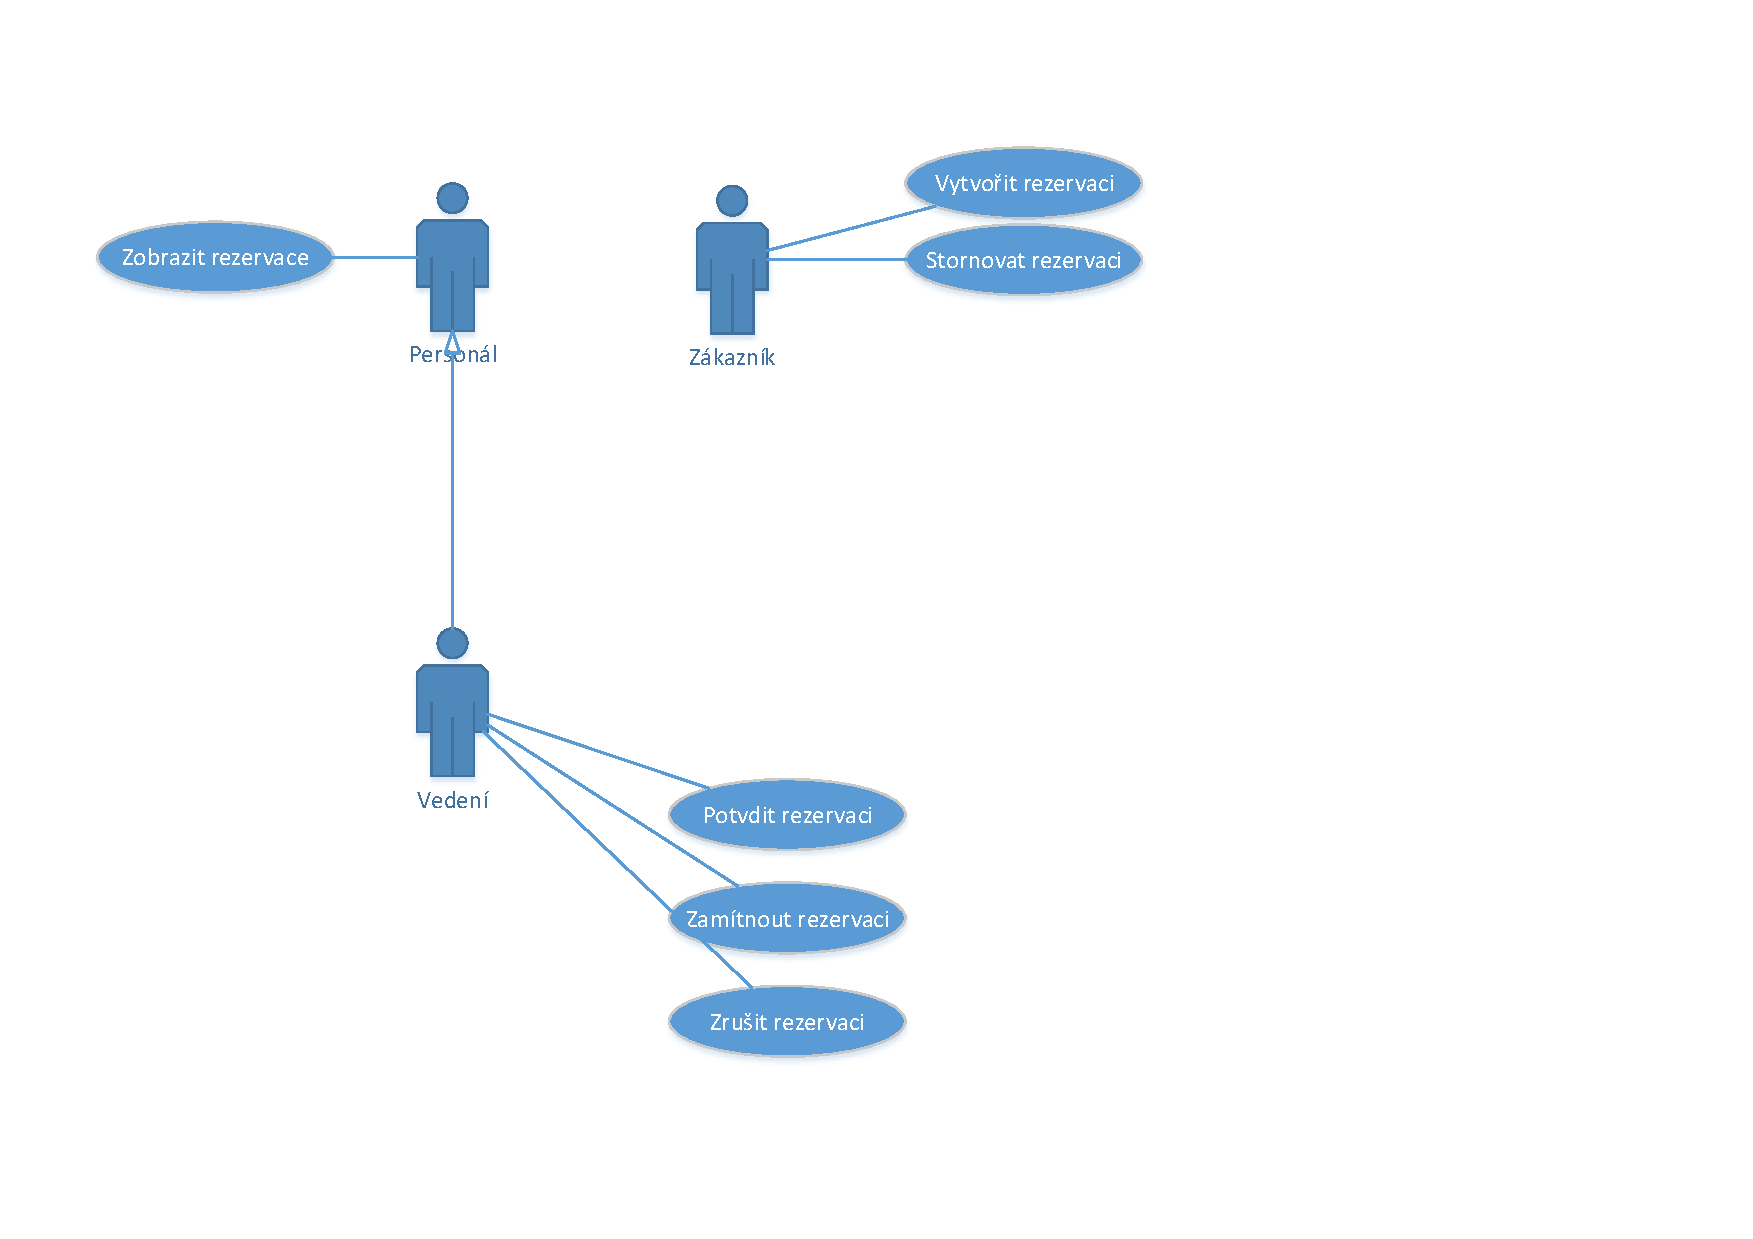
\includegraphics[scale=0.75]{resources/iteration01.pdf}
\captionof{figure}{Diagram použití v první iteraci}
\label{fig:iteration01}
\end{center}
\end{figure}

\newpage
\section*{Specifikace případů použití}
\textbf{Případ užití \uv{Vytvořit rezervaci}}

%%%%%%%%%%%%%%%%%%%%%%%
% Vytvoření rezervace %  
%%%%%%%%%%%%%%%%%%%%%%%
\begin{table}[ht!]
{\renewcommand{\arraystretch}{1.3}
\begin{tabular}{| r | p{12cm} |}
	\hline
	ID: & 1 \\
    \hline
    Název: & \textbf{Vytvořit rezervaci} \\
    \hline
    Vytvořeno: & Filip Kalous, Daniel Dušek, Anna Popková \\
    \hline
    Popis: & Uživatel vytvoří rezervaci \\
    \hline
    Primární aktéři: & Zákazník \\
    \hline
    Sekundární aktéři: & Systém \\
    \hline
    Předpoklady: & Žádné \\
    \hline
    Následné podmínky: & 
    \begin{minipage}[t]{0.75\textwidth}
    	\begin{enumerate}[nosep,after=\strut]
    		\item V systému je vytvořena zákazníkova rezervace.
    	\end{enumerate}
  	\end{minipage} \\
	\hline
    Akce pro spuštění: & Uživatel zvolí událost \uv{Vytvořit rezervaci} \\
    \hline
    Hlavní tok: & 
    \begin{minipage}[t]{0.75\textwidth}
    	\begin{enumerate}[nosep,after=\strut]
            \item Uživatel vyplní potřebné informace pro rezervaci
            \item Uživatel zvolí, zda chce salónek nebo konkrétní stůl
            \item Uživatel vyplní informace o své osobě
            \item Uživatel zvolí událost \uv{Potvrdit rezervaci}
    	\end{enumerate}
  	\end{minipage} \\
    \hline
    Alternativní toky: & 
    \begin{minipage}[t]{0.75\textwidth}
    	\begin{enumerate}[nosep,after=\strut]
            \item Uživatel vyplní potřebné informace pro rezervaci, ale systém mu sdělí, že restaurace je plně obsazena.
    	\end{enumerate}
  	\end{minipage} \\
    \hline
    Výjimky: & 
    \begin{minipage}[t]{0.75\textwidth}
    	\begin{enumerate}[nosep,after=\strut]
    		\item V době potvrzení rezervace je požadované místo již zabrané.
            \item Selhání načtení plánku restaurace
            \item Selhání systému
            \item Selhání operace
    	\end{enumerate}
  	\end{minipage} \\
    \hline
    Frekvence: & Často \\
    \hline
    Speciální požadavky: & 
    \begin{minipage}[t]{0.75\textwidth}
    	\begin{enumerate}[nosep,after=\strut]
    		\item Žádné
    	\end{enumerate}
  	\end{minipage} \\
    \hline

\end{tabular}}
\caption{Specifikace případu užití \uv{Vytvořit rezervaci}}
\label{table:1}
\end{table}


%%%%%%%%%%%%%%%%%%%%%%%%%%%%%%%%%%%
% Výjimka 1 - Vytvoření rezervace %  
%%%%%%%%%%%%%%%%%%%%%%%%%%%%%%%%%%%

\par{\textbf{Výjimky případu užití \uv{Vytvořit rezervaci}}}
\begin{table}[ht!]
{\renewcommand{\arraystretch}{1.3}
\begin{tabular}{| r | p{12cm} |}
	\hline
	ID: & 1.E.1 \\
    \hline
    Název: & \textbf{Vytvořit rezervaci: V době potvrzení rezervace je požadované místo již zabrané.} \\
    \hline
    Vytvořeno: & Filip Kalous, Daniel Dušek, Anna Popková \\
    \hline
    Popis: & Rezervace není potvrzena z důvodu zabraného místa. \\
    \hline
    Primární aktéři: & Systém \\
    \hline
    Sekundární aktéři: &  \\
    \hline
    Předpoklady: & V době potvrzování rezervace systém zjistí, že vybraná místa jsou již zarezervována.  \\
    \hline
    Následné podmínky: & 
	\begin{minipage}[t]{0.75\textwidth}
 		\begin{enumerate}[nosep,after=\strut]
 			\item Uživatel se nachází na stránce rezervačního formuláře.
 			\item Uživateli je zobrazena zpráva o neúspěchu vytvoření rezervace.
 		\end{enumerate}
    \end{minipage} \\
	\hline
    Akce pro spuštění: & Selhání rezervace. \\
    \hline
    Tok: & 
    \begin{minipage}[t]{0.75\textwidth}
    	\begin{enumerate}[nosep,after=\strut]
            \item Přesměrování uživatele zpět na rezervační formulář.
            \item Systém zobrazi chybovou hlášku o neúspěchu vytvoření rezervace.
    	\end{enumerate}
    \end{minipage} \\
    \hline
    Frekvence: & Zřídka \\
    \hline

\end{tabular}}
\caption{Vytvořit rezervaci: V době potvrzení rezervace je požadované místo již zabrané.}
\label{table:2}
\end{table}

%%%%%%%%%%%%%%%%%%%%%%%%%%%%%%%%%%%
% Výjimka 2 - Vytvoření rezervace %  
%%%%%%%%%%%%%%%%%%%%%%%%%%%%%%%%%%%
\begin{center}
\begin{table}[ht!]
{\renewcommand{\arraystretch}{1.3}
\begin{tabular}{| r | p{12cm} |}
	\hline
	ID: & 1.E.2 \\
    \hline
    Název: & \textbf{Vytvořit rezervaci: Selhání načtení plánku restaurace} \\
    \hline
    Vytvořeno: & Filip Kalous, Daniel Dušek, Anna Popková \\
    \hline
    Popis: & Systém nemůže načíst plánek restaurace. \\
    \hline
    Primární aktéři: & Systém \\
    \hline
    Sekundární aktéři: &  \\
    \hline
    Předpoklady: & 
    \begin{minipage}[t]{0.75\textwidth}
    	\begin{enumerate}[nosep,after=\strut]
    		\item Aplikace se snaží zobrazit neexistujíci (nesprávná) data.
    	\end{enumerate}
  	\end{minipage} \\
    \hline
    Následné podmínky: & 
    \begin{minipage}[t]{0.75\textwidth}
    	\begin{enumerate}[nosep,after=\strut]
    		\item Zobrazena chybová hláška
    	\end{enumerate}
  	\end{minipage} \\
	\hline
    Akce pro spuštění: & Selhání načtení plánku restaurace. \\
    \hline
    Tok: & 
    \begin{minipage}[t]{0.75\textwidth}
    	\begin{enumerate}[nosep,after=\strut]
        	\item Systém zobrazí chybvou hlášku.
            \item Systém se pokusí o znovunačtení plánku restaurace.
    	\end{enumerate}
  	\end{minipage} \\
    \hline
    Frekvence: & Zřídka \\
    \hline

\end{tabular}}
\caption{Vytvořit rezervaci: Selhání načtení plánku restaurace}
\label{table:3}
\end{table}
\end{center}
\newpage 
%%%%%%%%%%%%%%%%%%%%%%%%%%%%%%%%%%%
% Výjimka 3 - Vytvoření rezervace %  
%%%%%%%%%%%%%%%%%%%%%%%%%%%%%%%%%%%
\begin{center}
\begin{table}[ht!]
{\renewcommand{\arraystretch}{1.3}
\begin{tabular}{| r | p{12cm} |}
	\hline
	ID: & 1.E.3 \\
    \hline
    Název: & \textbf{Vytvořit rezervaci: Selhání systému} \\
    \hline
    Vytvořeno: & Filip Kalous, Daniel Dušek, Anna Popková \\
    \hline
    Popis: & Systém nedokáže pokračovat v případu. \\
    \hline
    Primární aktéři: & Systém \\
    \hline
    Sekundární aktéři: &  \\
    \hline
    Předpoklady: & 
    \begin{minipage}[t]{0.75\textwidth}
    	\begin{enumerate}[nosep,after=\strut]
    		\item Systém neprovedl korektně některý z kroku hlavního toku případu užití.
            \item Systém nespadl.
    	\end{enumerate}
  	\end{minipage} \\
    \hline
    Následné podmínky: & 
    \begin{minipage}[t]{0.75\textwidth}
    	\begin{enumerate}[nosep,after=\strut]
    		\item Systém nevytvořil rezervaci.
    	\end{enumerate}
  	\end{minipage} \\
	\hline
    Akce pro spuštění: & Selhání systému v libovolném místě toku případu \uv{Vytvořit rezervaci}. \\
    \hline
    Tok: & 
    \begin{minipage}[t]{0.75\textwidth}
    	\begin{enumerate}[nosep,after=\strut]
            \item Systém informuje uživatele chybovou hláškou o selhání.
            \item Systém přesměruje uživatele zpět na začátek rezervačního formuláře.
    	\end{enumerate}
  	\end{minipage} \\
    \hline
    Frekvence: & Zřídka \\
    \hline

\end{tabular}}
\caption{Vytvořit rezervaci: Selhání systému}
\label{table:4}
\end{table}
\end{center}


\newpage 
%%%%%%%%%%%%%%%%%%%%%%%%%%%%%%%%%%%
% Výjimka 4 - Vytvoření rezervace %  
%%%%%%%%%%%%%%%%%%%%%%%%%%%%%%%%%%%
\begin{center}
\begin{table}[ht!]
{\renewcommand{\arraystretch}{1.3}
\begin{tabular}{| r | p{12cm} |}
	\hline
	ID: & 1.E.4 \\
    \hline
    Název: & \textbf{Vytvořit rezervaci: Selhání operace} \\
    \hline
    Vytvořeno: & Filip Kalous, Daniel Dušek, Anna Popková \\
    \hline
    Popis: & Systém není schopen dokončit operaci potřebnou k úspěšnému dokončení případu užití. \\
    \hline
    Primární aktéři: & Systém \\
    \hline
    Sekundární aktéři: &  \\
    \hline
    Předpoklady: & 
    \begin{minipage}[t]{0.75\textwidth}
    	\begin{enumerate}[nosep,after=\strut]
    		\item Systém selhal ve vykonávání dílčí operace nezbytné pro dokončení kroku z hlavního toku případu užití.
            \item Systém nespadl, ale krok případu užití nebyl úspěšně dokončen.
    	\end{enumerate}
  	\end{minipage} \\
    \hline
    Následné podmínky: & 
    \begin{minipage}[t]{0.75\textwidth}
    	\begin{enumerate}[nosep,after=\strut]
    		\item Systém nedokončil krok úspěšně.
    	\end{enumerate}
  	\end{minipage} \\
	\hline
    Akce pro spuštění: & Selhání systému v libovolné dílčí operaci při vykonávání libovolného kroku toku případu použití. \\
    \hline
    Tok: & 
    \begin{minipage}[t]{0.75\textwidth}
    	\begin{enumerate}[nosep,after=\strut]
            \item Systém informuje uživatele chybovou hláškou o selhání.
            \item Systém přesměruje uživatele zpět na začátek kroku.
    	\end{enumerate}
  	\end{minipage} \\
    \hline
    Frekvence: & Zřídka \\
    \hline
\end{tabular}}
\caption{Vytvořit rezervaci: Selhání operace}
\label{table:4}
\end{table}
\end{center}


\newpage
%%%%%%%%%%%%%%%%%%%%%%%
% Zamítnout rezervaci %
%%%%%%%%%%%%%%%%%%%%%%%
\textbf{Případ užití \uv{Zamítnout rezervaci}}
\begin{center}
\begin{table}[ht!]
{\renewcommand{\arraystretch}{1.3}
\begin{tabular}{| r | p{12cm} |}
	\hline
	ID: & 2 \\
    \hline
    Název: & \textbf{Zamítnout rezervaci} \\
    \hline
    Vytvořeno: & Filip Kalous, Daniel Dušek, Anna Popková \\
    \hline
    Popis: & Kancelář zamítne uživatelem vytvořenou rezervaci. \\
    \hline
    Primární aktéři: & Kancelář \\
    \hline
    Sekundární aktéři: & Systém \\
    \hline
    Předpoklady: & Existuje rezervace, kterou není možné potvrdit. \\
    \hline
    Následné podmínky: & 
    \begin{minipage}[t]{0.75\textwidth}
    	\begin{enumerate}[nosep,after=\strut]
    		\item Rezervace je zamítnuta.
            \item Zákazník je informován o zamítnutí rezervace.
    	\end{enumerate}
  	\end{minipage} \\
	\hline
    Akce pro spuštění: & Kancelář zvolí akci \uv{Zamítnout rezervaci} \\
    \hline
    Hlavní tok: & 
    \begin{minipage}[t]{0.75\textwidth}
    	\begin{enumerate}[nosep,after=\strut]
    		\item Kancelář vybere rezervaci, kterou chce zamítnout.
            \item Kancelář popíše důvod zamítnutí rezervace.
            \item Kancelář potvrdí zamítnutí rezervace.
            \item Systém zašle informaci zákazníkovi o zamítnutí rezervace.
    	\end{enumerate}
  	\end{minipage} \\
    \hline
    Alternativní toky: & \\
    \hline
    Výjimky: & 
    \begin{minipage}[t]{0.75\textwidth}
    	\begin{enumerate}[nosep,after=\strut]
    		\item Selhání systému
    		\item Selhání operace
    	\end{enumerate}
  	\end{minipage} \\
    \hline
    Frekvence: & Velmi často \\
    \hline
    Speciální požadavky: & 
    \begin{minipage}[t]{0.75\textwidth}
    	\begin{enumerate}[nosep,after=\strut]
    		\item Žádné
    	\end{enumerate}
  	\end{minipage} \\
    \hline

\end{tabular}}
\caption{Specifikace případu užití \uv{Zamítnout rezervaci}}
\label{table:5}
\end{table}
\end{center}

\newpage
%%%%%%%%%%%%%%%%%%%%%%%%%%%%%%%%%%%
% Výjimka 1 - Zamítnutí rezervace %  
%%%%%%%%%%%%%%%%%%%%%%%%%%%%%%%%%%%
\textbf{Výjimka případu užití \textbf{Zamítnout rezervaci}}

\begin{table}[ht!]
{\renewcommand{\arraystretch}{1.3}
\begin{tabular}{| r | p{12cm} |}
	\hline
	ID: & 2.E.1 \\
    \hline
    Název: & \textbf{Zamítnutí rezervace: Selhání systému} \\
    \hline
    Vytvořeno: & Filip Kalous, Daniel Dušek, Anna Popková \\
    \hline
    Popis: & Systém nedokáže pokračovat v případu. \\
    \hline
    Primární aktéři: & Systém \\
    \hline
    Sekundární aktéři: &  \\
    \hline
    Předpoklady: & 
    \begin{minipage}[t]{0.75\textwidth}
    	\begin{enumerate}[nosep,after=\strut]
    		\item Systém neprovedl korektně některý z kroku hlavního toku případu užití.
            \item Systém nespadl.
    	\end{enumerate}
  	\end{minipage} \\
    \hline
    Následné podmínky: & 
    \begin{minipage}[t]{0.75\textwidth}
    	\begin{enumerate}[nosep,after=\strut]
    		\item Systém nepotvrdil zamítnutí rezervace.
            \item Je zobrazena chybová hláška.
    	\end{enumerate}
  	\end{minipage} \\
	\hline
    Akce pro spuštění: & Selhání systému v libovolném místě toku případu \uv{Vytvořit rezervaci} \\
    \hline
    Tok: & 
    \begin{minipage}[t]{0.75\textwidth}
    	\begin{enumerate}[nosep,after=\strut]
            \item Systém informuje uživatele chybovou hláškou o selhání.
            \item Systém přesměruje Vedení zpět na první krok zamítnutí rezervace.
    	\end{enumerate}
  	\end{minipage} \\
    \hline
    Frekvence: & Zřídka \\
    \hline

\end{tabular}}
\caption{Zamítnutí rezervace: Selhání systému}
\label{table:6}
\end{table}


\newpage
\textbf{Případ použití: \uv{Zrušit rezervaci}}
\begin{center}
\begin{table}[ht!]
{\renewcommand{\arraystretch}{1.3}
\begin{tabular}{| r | p{12cm} |}
	\hline
	ID: & 3 \\
    \hline
    Název: & \textbf{Zrušit rezervaci} \\
    \hline
    Vytvořeno: & Filip Kalous, Daniel Dušek, Anna Popková \\
    \hline
    Popis: & Zruší existující rezervaci \\
    \hline
    Primární aktéři: & Vedení \\
    \hline
    Sekundární aktéři: &  Zákazník \\
    \hline
    Předpoklady: & Existuje zákazníkem vytvořená a vedením potvrzená rezervace \\
    \hline
    Následné podmínky: & 
    \begin{minipage}[t]{0.75\textwidth}
    	\begin{enumerate}[nosep,after=\strut]
    		\item Rezervace je zrušena. 
            \item Aktér \uv{Zákazník} je o tom informován.
    	\end{enumerate}
  	\end{minipage} \\
    \hline
        Akce pro spuštění: & 
    	Aktér \uv{Vedení} restaurace v seznamu potvrzených rezervací klikne na tlačítko \uv{Zrušit rezervaci} u některého z existujících záznamů \\
    \hline
    Hlavní tok: & 
    \begin{minipage}[t]{0.75\textwidth}
    	\begin{enumerate}[nosep,after=\strut]
    		\item Systém zobrazí seznam potvrzených rezervací.
            \item Uživatel v seznamu potvrzených rezervací klikne na tlačítko zrušit rezervaci.
            \item Uživatel potvrdí, že zrušení rezervace.
            \item Systém zruší rezervaci a pošle zprávu na adresu zákazníka o zrušení rezervace.
    	\end{enumerate}
  	\end{minipage} \\
    \hline
    Alternativní toky: & \\ 
    \hline
    Výjimky: & 
    \begin{minipage}[t]{0.75\textwidth}
    	\begin{enumerate}[nosep,after=\strut]
    		\item Zákazník zruší rezervaci dříve než Vedení potvrdí, že chce rezervaci zrušit.
            \item Rušená rezervace již neexistuje. 
            \item Selhání operace
    	\end{enumerate}
  	\end{minipage} \\
    \hline
    Frekvence: & Málo časté \\
    \hline
    Speciální požadavky: & 
    \begin{minipage}[t]{0.75\textwidth}
    	\begin{enumerate}[nosep,after=\strut]
    		\item Vedení obdrželo prioritní požadavek na rezervaci konkrétního místa prostřednictvím kanálu mimo IS.
            \item Nemožnost použití místa, které je předmětem existující rezervace (například fyzické poškození).
    	\end{enumerate}
  	\end{minipage} \\
    \hline
\end{tabular}}
\caption{Specifikace případu užití \uv{Zrušit rezervaci}}
\label{table:7}
\end{table}
\end{center}


%%%%%%%%%%%%%%%%%%%%%%%%%%%%%%%%%
% Výjimka 1 - Zrušení rezervace %  
%%%%%%%%%%%%%%%%%%%%%%%%%%%%%%%%%
\newpage
\textbf{Výjimky případu užití \uv{Zrušit rezervaci}}
\begin{table}[ht!]
{\renewcommand{\arraystretch}{1.3}
\begin{tabular}{| r | p{12cm} |}
	\hline
	ID: & 3.E.1 \\
    \hline
    Název: & \textbf{Zrušit rezervaci: Zákazník zruší rezervaci dříve než Vedení potvrdí, že chce rezervaci zrušit.} \\
    \hline
    Vytvořeno: & Filip Kalous, Daniel Dušek, Anna Popková \\
    \hline
    Popis: & Rezervace kterou Vedení chce zrušit již byla zrušena. \\
    \hline
    Primární aktéři: & Vedení, Zákazník\\
    \hline
    Sekundární aktéři: &  Systém \\
    \hline
    Předpoklady: & Existuje potvrzená rezervace, kterou zákazník zrušil krátce před tím, než se rezervaci rozhodlo zrušit Vedení.  \\
    \hline
    Následné podmínky: & 
	\begin{minipage}[t]{0.75\textwidth}
 		\begin{enumerate}[nosep,after=\strut]
 			\item Vedení je informováno o tom, že rezervace již byla zrušena ze strany zákazníka.
 		\end{enumerate}
    \end{minipage} \\
	\hline
    Akce pro spuštění: & Kliknutí na tlačítko \uv{Zrušit rezervaci} v čase kdy rezervace již byla zrušena ze strany zákazníka.\\
    \hline
    Tok: & 
    \begin{minipage}[t]{0.75\textwidth}
    	\begin{enumerate}[nosep,after=\strut]
            \item Zobrazení informační hlášky o tom, že rezervace již byla zrušena ze strany zákazníka.
    	\end{enumerate}
    \end{minipage} \\
    \hline
    Frekvence: & Zřídka \\
    \hline

\end{tabular}}
\caption{Zrušit rezervaci: Zákazník zruší rezervaci dříve než Vedení potvrdí, že chce rezervaci zrušit.}
\label{table:8}
\end{table}

%%%%%%%%%%%%%%%%%%%%%%%%%%%%%%%%%
% Výjimka 2 - Zrušení rezervace %  
%%%%%%%%%%%%%%%%%%%%%%%%%%%%%%%%%
\begin{table}[ht!]
{\renewcommand{\arraystretch}{1.3}
\begin{tabular}{| r | p{12cm} |}
	\hline
	ID: & 3.E.2 \\
    \hline
    Název: & \textbf{Zrušit rezervaci: Rušená rezervace již neexistuje} \\
    \hline
    Vytvořeno: & Filip Kalous, Daniel Dušek, Anna Popková \\
    \hline
    Popis: & Rezervace kterou Vedení chce zrušit již v systému neexistuje. \\
    \hline
    Primární aktéři: & Vedení\\
    \hline
    Sekundární aktéři: &  Systém \\
    \hline
    Předpoklady: & V uživatelském rozhraní systému je zobrazena potvrzená rezervace, která již byla zrušena (například v jiném tabu prohlížeče). \\
    \hline
    Následné podmínky: & 
	\begin{minipage}[t]{0.75\textwidth}
 		\begin{enumerate}[nosep,after=\strut]
 			\item Vedení je informováno o tom, že rezervace již neexistuje.
            \item Neexistující položka zmizí z uživatelského rozhraní.
 		\end{enumerate}
    \end{minipage} \\
	\hline
    Akce pro spuštění: & Kliknutí na tlačítko \uv{Zrušit rezervaci} v čase kdy rezervace již v systému neexistuje.\\
    \hline
    Tok: & 
    \begin{minipage}[t]{0.75\textwidth}
    	\begin{enumerate}[nosep,after=\strut]
            \item Zobrazení informační hlášky o tom, že rezervace již v systému neexistuje.
            \item Odstranění neexistující rezervace z uživatelského rozhraní.
            \item Aktualizace uživatelského rozhraní pro odstranění dalších potenciálně neexistujících rezervací.
    	\end{enumerate}
    \end{minipage} \\
    \hline
    Frekvence: & Málo často \\
    \hline

\end{tabular}}
\caption{Zrušit rezervaci: Zákazník zruší rezervaci dříve než Vedení potvrdí, že chce rezervaci zrušit.}
\label{table:9}
\end{table}


%%%%%%%%%%%%%%%%%%%%%%%%%%%%%%%%%%%%%%%%%%%%%%%%%%%%%%
%                05 DOMAIN CLASS DIAGRAM             %
%%%%%%%%%%%%%%%%%%%%%%%%%%%%%%%%%%%%%%%%%%%%%%%%%%%%%%
\newpage
\begin{figure}[h!]
\begin{center}
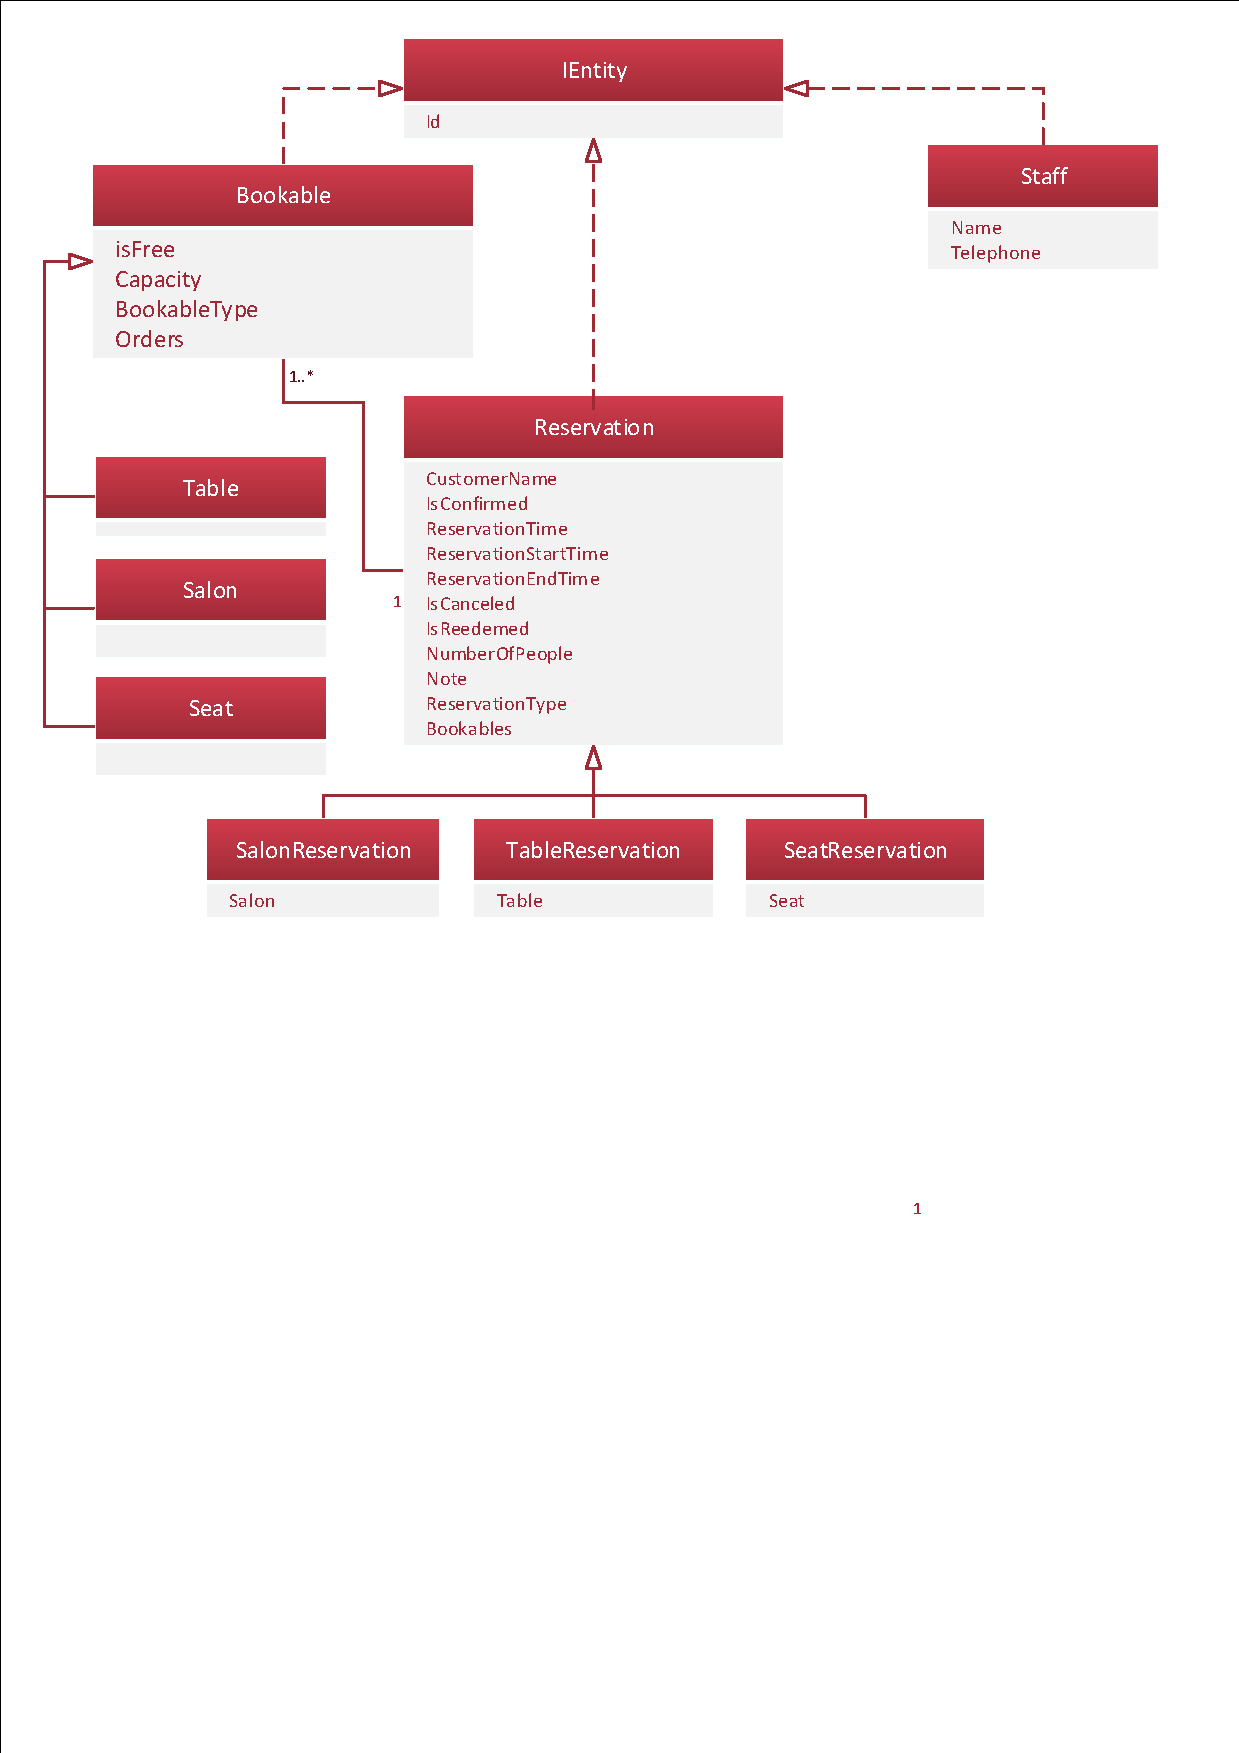
\includegraphics[scale=0.75]{../02_Vysledne_modely/05_1_ConceptualClassDiagram.pdf}
\vspace{-250pt}
\caption{Doménový konceptuální diagram tříd}
\label{fig:communication09-1}
\end{center}
\end{figure}